%
% BUS 338: Foundations of Innovation - A Course Overview
% Section: Introduction
%
% Author: Jeffrey Leung
%

\section{Introduction}
	\label{sec:introduction}
\begin{easylist}

& Business:
	&& Purpose is to create and reach a customer
	&& Composed of marketing and innovation

& \textbf{Invention:} Idea which is new, not immediately obvious, and useful
& \textbf{Innovation:} Translating an idea into goods or services with value
	&& Requires matching new ideas with marketal or societal needs

& Types of innovation:
	&& \textbf{Product/Service innovation:} Changing an offering to customers
	&& \textbf{Process innovation:} Changing the creation, composition, and/or maintenance of a product or service
		&&& Often in the interest of efficiency and cost
	&& \textbf{Position innovation:} Changing how an offering is portrayed in communications
	&& \textbf{Platform innovation:} Changing the foundation on which other businesses or processes operate
	&& \textbf{Business model (paradigm) innovation:} Changing the model of thought of the priorities and operations
		&&& E.g. RyanAir is a airline which provides low quality services at low costs
		&&& E.g. Netflix is a media streaming service which moved subscription services and distribution to online
	&& \textbf{Social innovation:} Creating solutions to social and/or environmental issues/deficits
		&&& Often target market weaknesses or address market failures
	&& \textbf{Sustainable innovation:}
		&&& Long-term maintenance of a concept or solution while creating the least environmental impact and utilizing all the possible resources

& Speed and impact of innovation:
	&& \textbf{Incremental/sustaining innovation:} Improvements to current performance with little effort required by the firm or customers (e.g. parking services)
	&& \textbf{Radical innovation:} Significant changes in a product (e.g. hybrid engine technology)
	&& \textbf{Disruptive innovation:} Large changes to the value proposition of a product and/or its perception by the market
		&&& E.g. Dyson's new bagless vacuum
	&& \textbf{Architectural innovation:} Changes to the composition and assembly of a product
	&& \textbf{Modular innovation:} Seamless substitution of a product for another product

& \textbf{Entrepreneur:} Person who creates a business, manages higher risks, and/or innovates

& Business Model Canvas: Method of mapping the value provided by a product and how the product is provided
	&& See \hyperref[sec:appendix-a]{Appendix A: Business Model Canvas}

& \textbf{Phases of Competition}: Diagram of how product innovation gives way to process innovation as a dominant design emerges
	&& When a product is created for a new purpose, the product is in a phase where it changes fluidly and product innovation occurs rapidly
	&& After a dominant design is chosen, the product is in a phase where product innovation decreases but process innovation occurs, with respect to the dominant design
	&& Over time, the product settles into a phase where the product is changing very little and has become specific, and the costs are low after significant process innovation
	&& See figure~\ref{fig:phases-of-competition}

\begin{figure}[h]
	\centering
	\caption{Phases of Competition}
	\label{fig:phases-of-competition}
	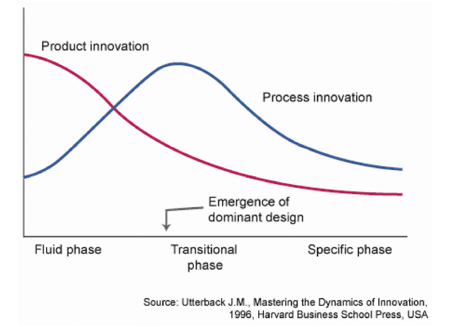
\includegraphics[width=0.7\textwidth]{phases-of-competition}
\end{figure}

\end{easylist}
\clearpage
